\section{Algorithms of Arithmetic}

\subsection{Lecture 1}

\subsubsection{Addition/Multiplication}

First, let us consider the problem of adding two $n$-bit numbers, $a$ and $b$. If both are a different amount of bits from each other,
we can pad 0's to the left of the smaller one until it reaches the length of the larger one (note that padding 0's doesn't change the sum).
The grade-school algorithm (add column-wise and do carries)
has to compute at most $n + 1$ additions, which we can assume are all constant-time. Thus, we say addition has complexity linear in $n$,
or $\Theta(n)$ (we drop the constant because 1 pales in significance to how great $n$ can grow).

But can we do better for addition? The answer is no; since it takes $n + 1$ bits to write our answer, any algorithm returning the sum
must require $n + 1$ operations. Thus, we say as a lower bound, addition is $\Omega(n)$ (the full definitions of these terms will come shortly).

Now we turn to the problem of multiplication. How fast is the grade school algorithm? First, we multiply digit-wise and then do a bunch of additions.
In binary, multiplying by a 0 or 1 and then right-padding with 0s (bitshifting) corresponds to a constant time operation for each bit of $b$.
Then, we have to add together $n$ potentially $2n$ bit numbers. This adds $n^2$ time. Thus, the runtime is quadratic in $n$
or $\Theta(n^2)$.

Now, can we do better for multiplication? It turns out we can. We do this by leveraging the idea of divide-and-conquer;
breaking our problem into smaller subproblems that we can solve recursively and then using these pieces to build the final solution.

Here is our first attempt:

\begin{algothm}[Naive Divide and Conquer]
    Suppose the numbers $x$ and $y$ that we wish to multiply are represented in decimal. Assume without loss of generality
    that both have the same number of digits $n$, and $n$ is a power of two (if they aren't then we can just pad with $0$s on the left
    until these requirements are met). Then, let $x_H$ be the upper half of the digits of $x$ and $x_L$ be the lower half of the digits of
    $x$ (and define $y_H, y_L$ analogously). Note that
    \begin{align*}
        x &= x_H \cdot 10^{n/2} + x_L \\
        y &= y_H \cdot 10^{n/2} + y_L \\
    \end{align*}
    And all the subscripted letters are $n/2$ digits long.
    Multiplying these together then yields:
    \[ x\cdot y = x_H \cdot y_H \cdot 10^n + (x_H \cdot y_L + x_L \cdot y_H) 10^{n/2} + x_L \cdot y_L \]
    Note that to do this multiplication, we have to do 3 $n$-digit additions as well as 4 $n/2$-digit multiplications
    (Multiplying by powers of 10 is just digit shifts, which can be done in linear time). To do the additions, let us use the
    standard grade school algorithm. To do the multiplications, let us have the function call itself recursively on the $n/2$-digit numbers.
    As a base case, note that if $x$ and $y$ are both one-digit numbers, the multiplication can be looked up in constant time.

    \textbf{Runtime Analysis} Now, to analyze the runtime, let the amount of time taken during the base case be $c'$ and let $c$ be another constant.
    Then, for the total running time $T(n)$, we know that:
    \[ T(n) = \begin{cases}
        4T(n/2) + cn & n > 1 \\
        c' & n = 1
    \end{cases} \]
    Since we make 4 recursive calls on an input of $n/2$ digits, and do a linear amount of work in every call. To analyze the runtime, we should draw
    a recursive tree.
    \\
    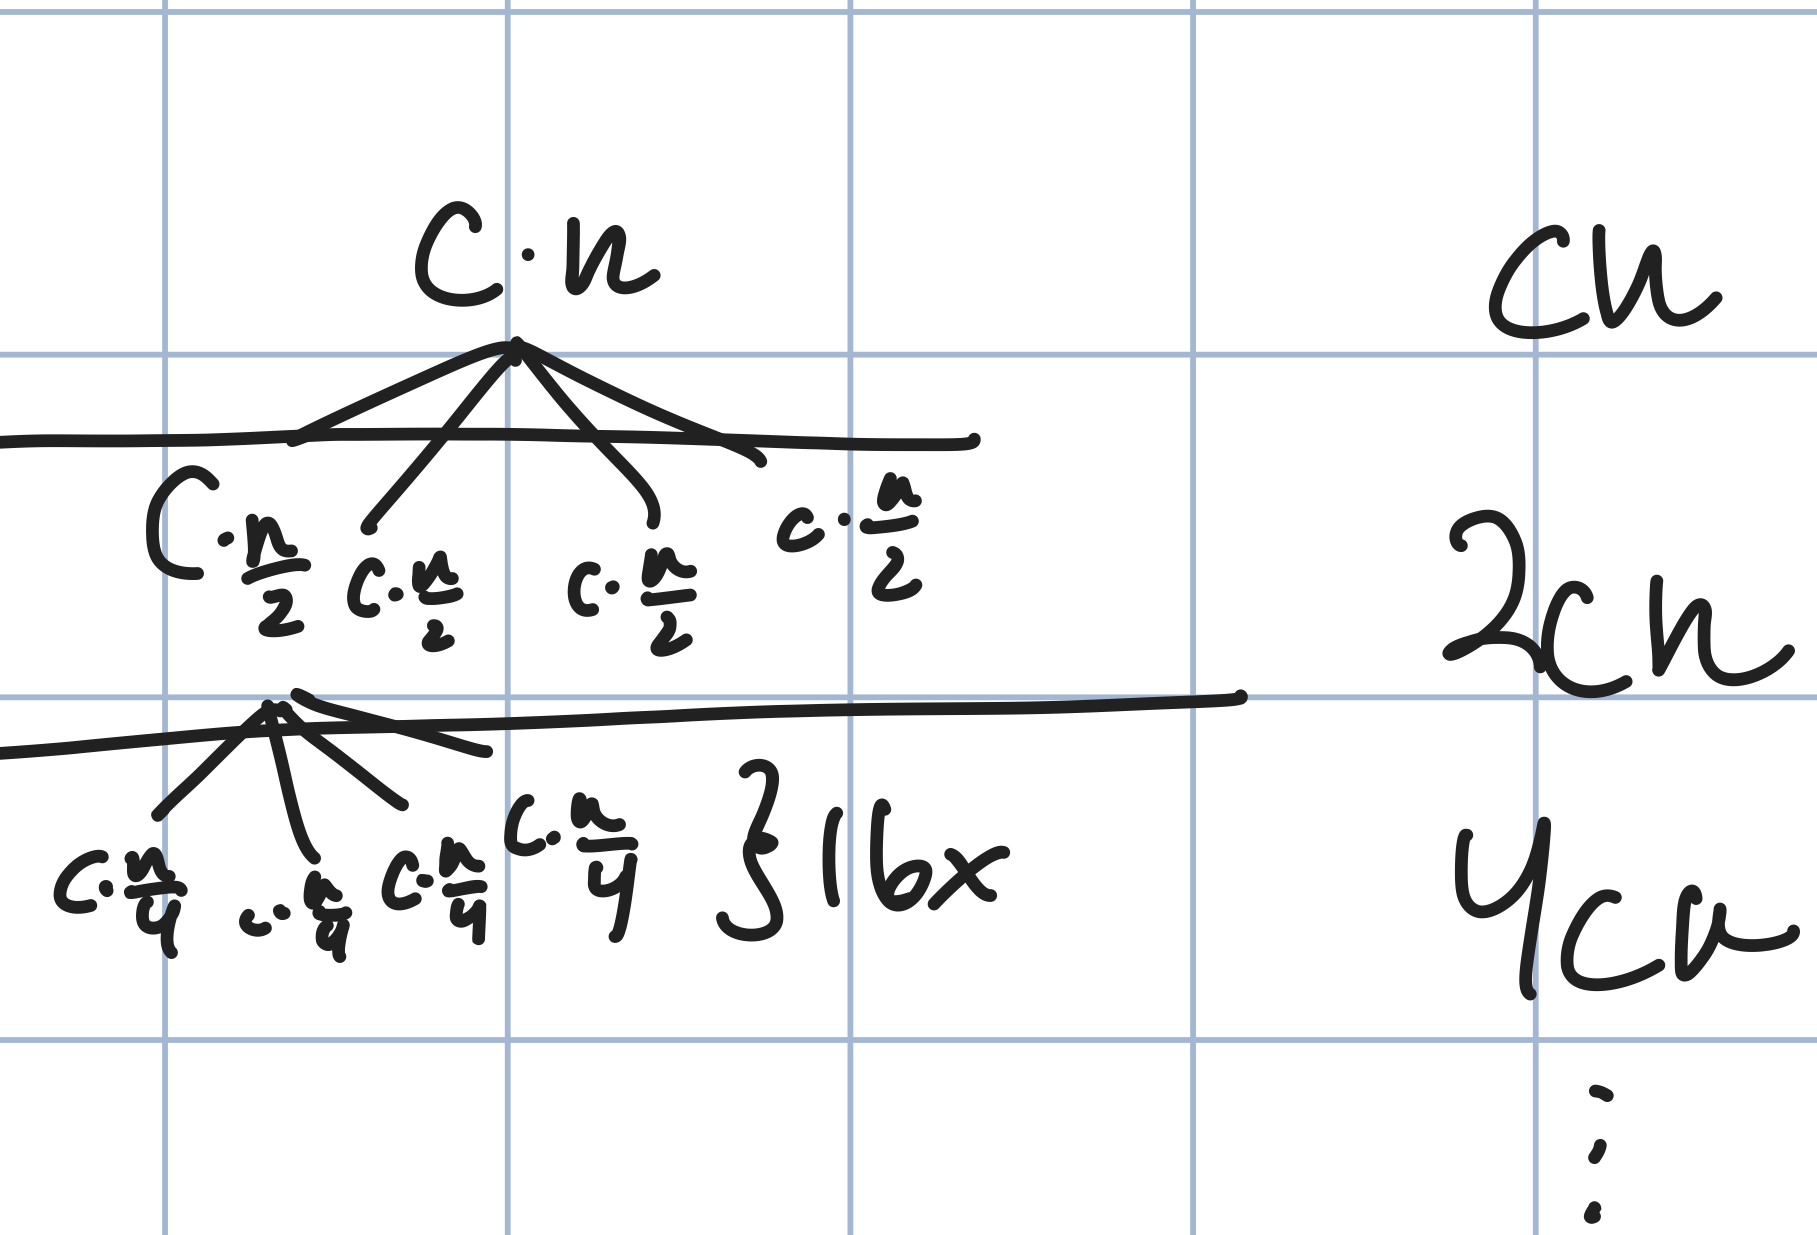
\includegraphics[width=80mm]{divide-conquer.png}

    Summing the nodes in this tree will give us the total runtime.
    As we can see from the diagram, on layer $i$ (considering the top layer as layer 0), there is $c \cdot n/2^i$
    work done at each node, and there are $2^{i + 1}$ nodes in that layer. Call $k = \log_2 n$. Then our total runtime is:
    \begin{align*}
        T(n) &= cn + 2cn + 4cn + \dots + 2^k  cn  \\
        &= cn \frac{2^{k + 1} - 1}{2 - 1} \\
        &\leq 2cn \cdot 2^k = 2cn^2 = \Theta(n^2)
    \end{align*}
    Thus, this algorithm is no better than our traditional grade-school algorithm.
\end{algothm}

However, there is a way to make this work. Gauss came up with a way to multiply two complex numbers (analogous to this setup) in
3 multiplications instead of 4. Similarly, Russian mathematician Karatsuba applied it to integer multiplication.

\begin{algothm}[Karatsuba's Algorithm for Multiplication]
    Proceed similarly to last time, defining $x_H, y_H, x_L, y_L$. However, define the following:
    \begin{align*}
        A = x_H \cdot y_H, B = x_L \cdot y_L, D = (x_L + x_H) \cdot (y_L + y_H)
    \end{align*}
    Then notice that the middle term from before is just $D - A - B$, i.e. we can write:
    \[ x \cdot y = A \cdot 10^n + (D - A - B) \cdot 10^{n/2} + B \]
    This means that we only need to compute three multiplications recursively (and do a few more additions, but since those take
    linear time, it's fine to have extra of those).

    \textbf{Runtime Analysis} The runtime analysis is similar to that of the naive algorithm. However, instead of the
    amount of work increasing by $4/2 = 2$ every level, instead the work will only increase by $3/2$ every time (3 subcalls of size $n/2$).
    Let us again define $k = log_2 n$. This gives us total runtime, $T(n)$, being:
    \begin{align*}
        T(n) &= cn + \frac{3cn}{2} + \frac{9cn}{2} + \cdots + \frac{3^k cn}{2^k} \\
        &= cn \frac{\qty(\frac{3}{2})^{k + 1} - 1}{\frac32 - 1} \\
        &\leq 2 \cdot {3}{2} cn \frac{3}{2}^k \\
        &= 3c 3^k \\
        &= 3c \qty(2^k)^{\log_2{3}} \\
        &= 3c n^{\log_2{3}} \\
        &= \mathcal{O}(n^{\log_2{3}})
    \end{align*}
    Note that $\log_2{3} \approx 1.585 < 2$, so this is better than our naive algorithm!
\end{algothm}

After Karatsuba's algorithm, people have continued to improve the worst case runtime of integer multiplication.
In 2019, a $\mathcal{O}(n \log n)$ algorithm was found for multiplying two numbers together. However, this series of algorithms
after Karatsuba's had such large constant factors that in practice, grade-school multiplication is still the one implemented most of the time.

As a note, Python currently uses Karatsuba multiplication, but only for numbers that are sufficiently large.